\section{Topologie}\label{sec:archi-topologie}
\renewcommand{\rightmark}{Topologie}

Cette section décrit et motive la topologie et les types de noeuds du réseau hybride IEEE 802.15.4-LoRa de capteurs. Cette toologie a été choisie pour correspondre au mieux au cas d'utilisation décrit dans l'introduction.\todo{REF INTRO}

\subsection*{Types de noeuds}
    Le protocole élaboré pour ce réseau hybride défini 3 types de noeuds:
    \begin{itemize}
        \item[-] La \textbf{racine LoRa} est la passerelle entre le réseau et un réseau IP externe. Elle possède donc une interface LoRa et par exemple une interface Wi-Fi.
        \item[-] La \textbf{racine RPL}, comme son l'indique, est la racine d'un réseau RPL. Elle possède également une interface LoRa pour communiquer avec la racine LoRa.
        \item[-] Les \textbf{noeuds RPL} sont des noeuds du réseau RPL.
    \end{itemize}

\subsection*{Topologie}
Comme l'illustre la figure~\ref*{fig:archi-topologie} la topologie choisie est une topologie mixte.

On a d'abord un ensemble de réseaux RPL possèdant chacun un préfixe IP attribué par la racine LoRa. Dans lesquels les communications sont réalisées par des liens IEEE 802.15.4.
De part l'utilisation de RPL, chaque réseaux forme un DODAG.

Ensuite, chaque réseau RPL est connecté à la racine LoRa via sa racine. Les liens entre les racines RPL et la racine LoRa forment une topologie en étoile.

Ce choix de topoligie offre plusieurs avantages: Le fait d'avoir un ensemble de réseaux RPL implique qu'il n'y a pas qu'une seule racine RPL et donc pas qu'un seule de défaillance; L'administration du réseau est simplifiée. En effet, un réseau RPL pourraît, par exemple, correspondre à une parcelle de terrain. 

L'inconvéninent de cette topologie est que la racine LoRa constitue un seul point de défaillance. Une solution plus robuste qui a été envisagée, est d'avoir un réseau maillé avec les racines RPL et les racines LoRa. Cependant, une telle architecture est difficile à mettre en oeuvre car le protocole MAC a établir pour les liens LoRa est plus complexe et nécessite un protocole de routage.

\begin{figure}[H]
    \centering
    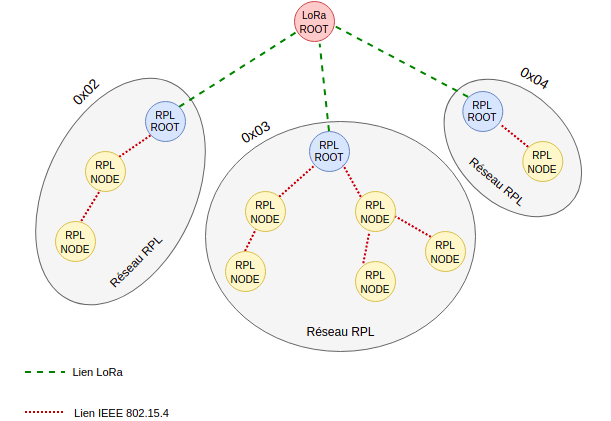
\includegraphics[scale=0.7]{res/pictures/loramac-topologie.drawio.png}
    \caption{Topologie du réseau hybride.}
    \label{fig:archi-topologie}
\end{figure}